\begin{center}

\begin{tikzpicture}[font=\small,overlay,
mycirclex/.style={draw, circle, minimum size=1.0em, inner sep = 0.2mm}, 
mydiamond/.style={draw, diamond, minimum size=0.78em, inner sep = 0mm}, 
myrectang/.style={draw, rectangle, minimum size=0.60em, inner sep = 0mm}, 
>=stealth]

\definecolor{mygreen}{rgb}{0, 0.7, 0}
\definecolor{myyellow}{rgb}{0.8, 0.6, 0}

\def\colx{black}
\def\cola{red} 
\def\colb{blue}
\def\colc{violet}
\def\cold{cyan} 
\def\cole{myyellow}
\def\colf{brown}


\def\len{2.0cm}

% G1
\begin{scope}[local bounding box=bbox, xshift=-6.0cm]
\path<1-> node[mycirclex] (v1) at (1.0 * \len, 0) {$s$};
\path<1-> node[mycirclex] (v2) at (2.0 * \len, 0) {$a$};
\path<1-> node[mycirclex] (v3) at (3.0 * \len, 0) {$b$};
\path<1-> node[mycirclex] (v4) at (4.0 * \len, 0) {$c$};
\path<1-> node[mycirclex] (v5) at (5.0 * \len, 0) {$t$};

\path<1-> [draw, \colx, ->, line width=0.04cm] (v1) -- (v2);
\path<1-> [draw, \colx, ->, line width=0.04cm] (v2) -- (v3);
\path<1-> [draw, \cola, ->, line width=0.04cm] (v3) -- (v4);
\path<1-> [draw, \colx, ->, line width=0.04cm] (v4) -- (v5);

\path<1-> [draw, \cola, ->, line width=0.04cm, bend left = 40] (v1) to (v3);
\path<1-> [draw, \colx, ->, line width=0.04cm, bend left = 40] (v3) to (v5);
\path<1-> [draw, \colx, ->, line width=0.04cm, bend left = 40] (v2) to (v4);

\path<1-> node[\colx] at (1.5 * \len, 0.18cm) {$e_1$};
\path<1-> node[\colx] at (2.5 * \len, 0.18cm) {$e_2$};
\path<1-> node[\cola] at (3.5 * \len, 0.18cm) {$e_3$};
\path<1-> node[\colx] at (4.5 * \len, 0.18cm) {$e_4$};

\path<1-> node[\cola] at (2.0 * \len, 1.0cm) {$e_5$};
\path<1-> node[\colx] at (3.0 * \len, 1.0cm) {$e_6$};
\path<1-> node[\colx] at (4.0 * \len, 1.0cm) {$e_7$};

\end{scope}
%\path<1-> [draw, rounded corners] ($(bbox.south west) - (0.00cm, 0.25cm)$) rectangle ($(bbox.north east) + (0.1cm, 0)$);
%\node at ($(bbox.south) - (0.00cm, 0.2cm)$) [label=below:{$G_2 - G_1 = \{c\}$}]{};

\path<1-> [draw, line width=0.1cm, ->] (0.0cm, -0.9cm) -- (0.0cm, -1.5cm);

% G2
\begin{scope}[local bounding box=bbox, xshift=-6.0cm, yshift=-3.5cm]
\path<1-> node[mycirclex] (v1) at (1.0 * \len, 0) {$s$};
\path<1-> node[mycirclex] (v2) at (2.0 * \len, 0) {$a$};
\path<1-> node[mycirclex] (v3) at (3.0 * \len, 0) {$b$};
\path<1-> node[mycirclex] (v4) at (4.0 * \len, 0) {$c$};
\path<1-> node[mycirclex] (v5) at (5.0 * \len, 0) {$t$};

\path<1-> [draw, \colx, ->, line width=0.04cm] (v1) -- (v2);
\path<1-> [draw, \colx, ->, line width=0.04cm] (v2) -- (v3);
\path<1-> [draw, \colx, ->, line width=0.04cm] (v4) -- (v5);

\path<1-> [draw, \cola, ->, line width=0.04cm, bend left = 40] (v1) to (v4);
\path<1-> [draw, \colx, ->, line width=0.04cm, bend left = 40] (v3) to (v5);
\path<1-> [draw, \colx, ->, line width=0.04cm, bend left = 40] (v2) to (v4);

\path<1-> node[\colx] at (1.5 * \len, 0.18cm) {$e_1$};
\path<1-> node[\colx] at (2.5 * \len, 0.18cm) {$e_2$};
\path<1-> node[\colx] at (4.5 * \len, 0.18cm) {$e_4$};

\path<1-> node[\cola] at (2.5 * \len, 1.4cm) {$e_8$};
\path<1-> node[\colx] at (3.0 * \len, 1.0cm) {$e_6$};
\path<1-> node[\colx] at (4.0 * \len, 1.0cm) {$e_7$};

\end{scope}

\end{tikzpicture}
\end{center}
